\subsection*{Overview}
For my fifth experiment, I decided to take inspiration from
\textcite{yanaiFood}, where pre-training was used training a model for food
classification. In order to achieve this, I retrained the final layer of the
Inception V3 model which was trained on the ImageNet dataset. This is called
Transfer Learning. I followed the tutorial by Google on the tensorflow website
for direction on this process \textcite{retrainInception}.

Firstly, in order to retrain the final layer of a model, a dataset must be
prepared in the correct way. I used the Food-101 dataset \textcite{food101}
which I will analyse in a later section. The dataset must be structured so that
there is a separated directory for each class with the directory name as the class
name. These directories should contain all the images for this class. 

Once this dataset has been set up correctly, a directory can be found on github
which contains the necessary files for this tutorial. When the directory has
been downloaded, the following command can be ran:
\begin{lstlisting}
python tensorflow/examples/image_retraining/retrain.py \ --image_dir
~/dataset_directory
\end{lstlisting}

The first thing that the script will do is create bottleneck files for the
images. A bottleneck is a term used to define the final layer before the output
layer. This is so that for each image, we do not have to push it through the
entire network during training \textcite{retrainInception}.

After, the bottlenecks are created, the training can be completed. The images
are split into three sub directories of training, testing and validation. By
default, these images are split into percentages of 80\%, 10\% and 10\%
respectively. The model is trained at a default of 4000 steps. 

The command used for using this model once it is trained is:
\begin{lstlisting}
python tensorflow/examples/label_image.py --graph=/tmp/output_graph.pb
--labels=/tmp/output_labels.txt --input_layer=Mul --output_layer=final_result
--input_mean=128 --input_std=128 --image=~/image_directory
\end{lstlisting}

\subsection*{Network Architecture}
The Inception V3 model network architecture was used which consists of 22
layers.

\subsection*{Dataset}
The dataset used for this experiment is the Food-101 dataset \textcite{Food
101}. This dataset has 101 classes with 1000 images for each class.

\subsection*{Libraries}
Tensorflow and Numpy were used to run this scipt.

\subsection*{Script}
The following snippets of code are from the retrain.py script.

\begin{lstlisting}
# Add the new layer that we'll be training.
(train_step, cross_entropy, bottleneck_input, ground_truth_input,
final_tensor) = add_final_training_ops(
            len(image_lists.keys()), FLAGS.final_tensor_name,
            bottleneck_tensor,
            model_info['bottleneck_tensor_size'],
            model_info['quantize_layer'])
 
# Create the operations we need to evaluate the accuracy of our new layer.
evaluation_step, prediction = add_evaluation_step(
final_tensor, ground_truth_input)
 
# Merge all the summaries and write them out to the summaries_dir
merged = tf.summary.merge_all()
train_writer = tf.summary.FileWriter(FLAGS.summaries_dir + '/train',
                                     sess.graph)
 
validation_writer = tf.summary.FileWriter(
    FLAGS.summaries_dir + '/validation')
 
# Set up all our weights to their initial default values.
init = tf.global_variables_initializer()
sess.run(init)

\end{lstlisting}




\begin{lstlisting}
# We've completed all our training, so run a final test evaluation on
# some new images we haven't used before.
test_bottlenecks, test_ground_truth, test_filenames = (
    get_random_cached_bottlenecks(
        sess, image_lists, FLAGS.test_batch_size, 'testing',
        FLAGS.bottleneck_dir, FLAGS.image_dir, jpeg_data_tensor,
        decoded_image_tensor, resized_image_tensor, bottleneck_tensor,
        FLAGS.architecture))
test_accuracy, predictions = sess.run(
   [evaluation_step, prediction],
   feed_dict={bottleneck_input: test_bottlenecks,
        ground_truth_input: test_ground_truth})
tf.logging.info('Final test accuracy = %.1f%% (N=%d)' %
                (test_accuracy * 100, len(test_bottlenecks)))
\end{lstlisting}

\subsection*{Results}
The final test accuracy for this retrained model was 54.8\%.

For example, an image of pizza, see \ref{fig:pizza} was fed into the model with the followng results:
\begin{itemize}
    \item{pizza 0.925}
    \item{pancakes 0.008}
    \item{nachos 0.007}
    \item{beef carpaccio 0.006}
    \item{tiramisu 0.004}
\end{itemize}

\begin{figure}
     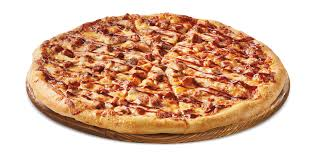
\includegraphics{pizza}
     \caption{Pizza}
     \label{fig:pizza}
\end{figure}

\subsection*{Analysis}
